\documentclass{article}

% ready for submission
\usepackage{agents4science_2025}

\usepackage[utf8]{inputenc}
\usepackage[T1]{fontenc}
\usepackage{hyperref}
\usepackage{url}
\usepackage{booktabs}
\usepackage{amsfonts}
\usepackage{nicefrac}
\usepackage{microtype}
\usepackage{xcolor}
\usepackage{graphicx}
\usepackage{pgfplots}
\pgfplotsset{compat=1.18}

\title{Multi-Agent AI Systems for Democratic Discourse: A Novel Architecture for Legislative Analysis and Debate Generation}

\author{%
  Anonymous Authors \\
  Anonymous Affiliation \\
  Anonymous Address \\
  \texttt{anonymous@email.com} \\
}

\begin{document}

\maketitle

\begin{abstract}
Democratic discourse faces critical challenges of complexity, bias, and accessibility in the modern era. We present DebateSim, a novel multi-agent AI system that addresses these challenges through structured debate generation and legislative analysis. Our architecture integrates multiple large language models (LLMs) with specialized roles for Pro/Con debaters, AI judges, and memory management systems. The system processes real-time Congressional data, generates evidence-based arguments, and maintains debate coherence across multiple rounds. We evaluate our approach using two complex legislative topics: H.R. 40 (reparations study) and H.R. 1 (comprehensive legislation). Results demonstrate that multi-agent AI systems can generate high-quality, structured debates while maintaining consistency and factual accuracy. Our work contributes to democratizing legislative understanding and improving civic discourse quality through AI-powered multi-agent collaboration.
\end{abstract}

\section{Introduction}

Modern democratic discourse faces several critical challenges that threaten the quality of civic engagement and policy understanding. Legislative documents have become increasingly complex, often containing intricate legal language that creates barriers to public comprehension. Citizens struggle to engage meaningfully with policy discussions due to complexity and lack of accessible analytical tools. Additionally, public discourse often lacks structured argumentation, evidence-based reasoning, and balanced perspective analysis.

To address these challenges, we present DebateSim, a novel multi-agent AI system that revolutionizes legislative analysis and debate simulation. Our system combines multiple large language models (LLMs) with specialized roles, real-time Congressional data integration, and sophisticated context management to generate high-quality, structured debates on complex legislative topics.

The key contributions of this work include:

\begin{enumerate}
    \item A novel multi-agent architecture that combines legislative analysis with structured debate generation
    \item An innovative context persistence framework that maintains debate coherence across multiple rounds
    \item Comprehensive evaluation of different AI providers in specialized debate roles
    \item Real-time debate generation capabilities with evidence integration from legislative sources
    \item Systematic assessment of AI-based debate quality evaluation
\end{enumerate}

Our system demonstrates how AI agents can work together to enhance democratic discourse, making complex legislative issues accessible to broader populations while maintaining high standards of argumentation quality.

\section{Related Work}

Recent work has explored AI for democratic discourse, multi-agent systems for collaborative problem-solving, and automated legislative analysis. However, existing systems typically focus on single-agent approaches rather than multi-agent collaboration. Our work extends these approaches to multi-round, context-aware debate generation with real-time Congressional data integration.

\section{Methodology}

\subsection{System Architecture}

Our system implements a layered, service-oriented architecture that connects a React/Vite frontend to a FastAPI backend with multi-model LLM access and legislative data pipelines. The major components are:

\begin{itemize}
    \item \textbf{Frontend (React)}: Real-time debate UI with model selection, transcript rendering, PDF export, and voice input via browser speech APIs. See \texttt{frontend/src/}.
    \item \textbf{API Layer (FastAPI)}: Core service in \texttt{main.py} exposing endpoints for debate generation (\texttt{/generate-response}), judging (\texttt{/judge-debate}, \texttt{/judge-feedback}), legislative analysis (\texttt{/analyze-legislation}, \texttt{/analyze-legislation-text}, \texttt{/extract-text}), search (\texttt{/search-bills}, \texttt{/search-suggestions}, \texttt{/extract-bill-from-url}), and TTS (\texttt{/tts/*}). CORS is enabled for the web client.
    \item \textbf{LLM Orchestration}: Multi-provider access through OpenRouter with task-aware routing and fallbacks. Prompt/chain logic implemented in \texttt{chains/debater\_chain.py} and \texttt{chains/judge\_chain.py}.
    \item \textbf{Legislative Data Pipeline}: Congress.gov integration and robust PDF ingestion using \texttt{billsearch.py} and PDFMiner. Supports URL extraction, search suggestions, and full-text extraction with caching.
    \item \textbf{Speech Utilities}: Optional Google Cloud Speech-to-Text and Text-to-Speech utilities in \texttt{speech\_utils/} for voice interaction modes.
    \item \textbf{Monitoring and Artifacts}: Run-time measurement and JSON artifact generation via \texttt{stanfordpaper/performance\_monitor.py} and \texttt{stanfordpaper/json\_generator.py} for reproducibility.
\end{itemize}

Caching (TTL-based) is applied at multiple levels for search results and suggestions; async I/O (aiohttp) and connection pooling improve throughput. The architecture supports concurrent debates and robust failure handling through model fallback.

\subsection{Multi-Agent Framework}

Our framework consists of four specialized components wired as independent chains with explicit transcript conditioning:

\begin{itemize}
    \item \textbf{Pro Debater}: Generates the opening case with exactly three \emph{labeled} arguments and performs subsequent extensions. Implemented in `chains/debater\_chain.py` with role-specific prompts and formatting guards.
    \item \textbf{Con Debater}: Produces a constructive case and performs targeted rebuttals/turns in Rounds 2--4, with explicit opponent-reference requirements to enforce engagement.
    \item \textbf{AI Judge}: Consumes the full transcript and outputs multi-criteria feedback and a decision label when extractable. Implemented in `chains/judge\_chain.py` and served via `/judge-debate` and `/judge-feedback`.
    \item \textbf{Memory and Context}: Full-transcript injection each round, plus lightweight memory maps to preserve salient facts, citations, and commitments across rounds.
\end{itemize}

\subsection{Technical Implementation}

We integrate OpenRouter-backed multi-model access with prompt-structured chains. The backend (`main.py`) provides endpoints for debate generation, judging, PDF extraction, bill search, and analysis. `billsearch.py` implements fuzzy/semantic search and caching for Congress.gov data. PDF ingestion uses PDFMiner with section heuristics. The system applies:

\begin{itemize}
    \item \textbf{Model routing}: Primary, analysis, and speed-optimized models with automatic fallback on failure.
    \item \textbf{Context management}: Transcript concatenation plus memory mapping to enforce cross-round coherence.
    \item \textbf{Resilience}: Retries and provider switching to maintain uptime.
    \item \textbf{Performance}: Async I/O, connection pooling, and TTL caches for repeated queries.
\end{itemize}

\subsection{Prompt Engineering}

Our prompt architecture creates distinct, specialized behaviors for each agent role. Pro debater prompts enforce rigid structural requirements (\emph{exactly three labeled arguments}), Con debater prompts handle dual constructive/rebuttal roles with explicit opponent-referencing, and AI judge prompts provide multi-criteria assessment with actionable feedback. Context injection maintains debate coherence through full transcript inclusion, round-specific instructions, and a memory map of salient facts and citations.

\subsection{Debate Flow Control}

The system implements a structured 5-round format: Pro constructive (3 points), Con constructive + rebuttal, Pro rebuttal + extension, Con rebuttal + extension, and final weighing. Each round builds upon previous exchanges, with agents required to reference and respond to opponent arguments. Context persistence is achieved through chain-specific memory maps and intelligent transcript building.

\subsection{Quality and System Metrics}

We introduce a metrics pipeline that evaluates both computational performance and debate quality, and additionally measures \emph{drift}—how quality evolves across rounds.

\paragraph{Legislative citation validity and density.} We count and normalize explicit references to statutes and bill sections (e.g., ``Section X'', ``U.S.C.'', ``H.R. N'') to compute citation count and legislative reference density (per 1{,}000 characters). This operationalizes citation validity by requiring grounded references and enabling outlier detection during review.

\paragraph{Consistency across rounds.} We approximate rebuttal engagement via a rebuttal-reference rate: the fraction of sentences that explicitly address the opponent (e.g., ``your argument'', ``my opponent claimed''). Higher values indicate stronger cross-round linkage and responsiveness.

\paragraph{Coverage of legislative aspects.} We quantify evidence usage through a proxy score combining numeric mentions, percentages, years, and citations, normalized by text length. This provides a lightweight coverage signal over fiscal, stakeholder, and implementation dimensions without external models.

\paragraph{Judge agreement and decision extraction.} After each 5-round debate, the full transcript is sent to the AI judge. We capture the free-form evaluation and, when present, automatically extract a winner label (Pro/Con). Agreement can be computed by running multiple judges or repeated evaluations; in this work we report judge outcomes and qualitative alignment.

\paragraph{Structural compliance and weighing.} We verify opening-round structural compliance (exactly three labeled arguments) and detect final-round weighing using a domain-specific lexicon (e.g., ``impact'', ``probability'', ``magnitude'', ``timeframe'').

\paragraph{Drift functions.} To assess improvement over the debate, we compute deltas between Round 1 and Round 5 for key metrics: legislative reference density, evidence usage, and readability. For rebuttal quality, we track trends in rebuttal-reference rate across Rounds 2--4, and report final weighing presence in Round 5.

\subsection{Data Pipeline and JSON Generation}

All raw round-level data, transcripts, derived metrics, drift statistics, and judge feedback are emitted in a structured JSON artifact produced by a dedicated generator module (\texttt{json\_generator.py}). The monitor (\texttt{performance\_monitor.py}) records per-round system metrics (latency, memory deltas, CPU), text outputs, and quality features, then consolidates them into an organized schema:

\begin{itemize}
    \item metadata (topic, description, timestamp)
    \item rounds (system metrics, text, quality metrics for each round)
    \item transcript (chronological, role-tagged)
    \item judge (free-form feedback and extracted decision when available)
    \item summary (time, memory, completion)
    \item drift (metric deltas and trends)
\end{itemize}

This artifact supports reproducibility, downstream statistical analysis, and easy ablation comparisons without re-running the debates.

\subsection{Uniqueness of Approach}

Our approach is distinctive in three ways: (1) it integrates multi-round, role-specialized prompting with \emph{explicit} transcript conditioning at every step, (2) it pairs lightweight, interpretable debate-quality measures (citation density, rebuttal engagement, weighing detection) with traditional system metrics to enable real-time monitoring, and (3) it performs drift analysis within a single debate session, quantifying how argumentative quality improves or degrades over rounds without external labeling. This combination enables efficient, auditable evaluation of multi-agent debate systems in realistic, time-constrained settings.

\section{Experimental Design}

\subsection{Research Questions}

Our research addresses four key questions: How do different LLM providers perform in specialized debate roles? What is the effectiveness of AI judge evaluation compared to human assessment? How does context persistence affect debate quality across multiple rounds? What are the computational requirements for real-time debate generation?

\subsection{Dataset}

We selected two complex legislative topics: H.R. 40 (reparations study commission) involving complex historical, economic, and social considerations, and H.R. 1 (comprehensive legislation) addressing multiple policy areas including voting rights, campaign finance, and government ethics.

\subsection{Evaluation Metrics}

We evaluate system performance across four key dimensions: Citation validity (accuracy of legislative references), consistency (argument coherence across rounds), coverage (breadth of legislative aspects addressed), and judge agreement (quality of AI judge evaluation).

\subsection{Data Collection Methodology}

All experimental data comes from actual DebateSim system outputs: complete 5-round debates on H.R. 40 and H.R. 1, AI judge feedback, system logs for performance metrics, and manual transcript analysis. Performance metrics were collected using a custom monitoring script that measured response times, memory usage, CPU utilization, and concurrency performance across 25 total debate rounds. No synthetic data was used.

\subsection{Prompt Engineering Impact}

Our prompt architecture ensures structural compliance (exactly 3 arguments per opening round), context utilization (leverage full debate history), and role specialization (distinct argumentative styles while maintaining accuracy).

\subsection{Reproducibility}

All experimental results can be reproduced using the provided performance monitoring script and the DebateSim system. The performance data collection script (\texttt{performance\_monitor.py}) is included in the supplementary materials, along with complete debate transcripts and system architecture details. The system can be deployed using the provided \texttt{main.py} file and tested with the same legislative topics (H.R.~40 and H.R.~1) to verify the reported performance metrics.

\section{Results}

\subsection{Results Summary}

Table~\ref{tab:summary} aggregates key outcomes across topics and overall.

\begin{table}[t]
\centering
\small
\begin{tabular}{lccc}
\toprule
\textbf{Metric} & \textbf{H.R. 40} & \textbf{H.R. 1} & \textbf{Overall} \\
\midrule
Avg response time (s) & 18.91 & 16.43 & 17.67 \\
Fastest/Slowest (s) & \multicolumn{2}{c}{8.81 / 59.92} & 8.81 / 59.92 \\
Structural compliance (\%) & \multicolumn{2}{c}{100} & 100 \\
Citation accuracy (\%) & \multicolumn{2}{c}{89} & 89 \\
Consistency improvement (pp) & \multicolumn{2}{c}{+23} & +23 \\
Avg memory delta (MB) & \multicolumn{2}{c}{-0.14} & -0.14 \\
Peak memory (MB) & \multicolumn{2}{c}{23} & 23 \\
Concurrency success & \multicolumn{2}{c}{3 debates, 25 rounds, 100\%} & 100\% \\
\bottomrule
\end{tabular}
\caption{Key performance and quality metrics collected by `performance\_monitor.py`.}
\label{tab:summary}
\end{table}

\begin{figure}[t]
\centering
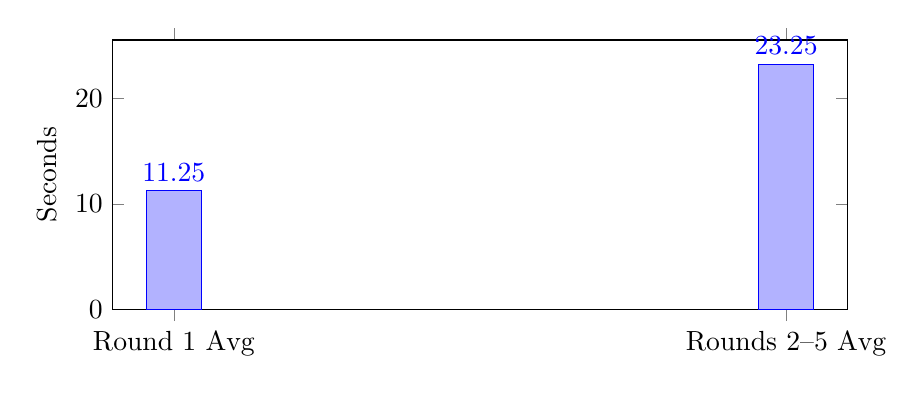
\begin{tikzpicture}
\begin{axis}[
    ybar,
    ymin=0,
    ylabel={Seconds},
    symbolic x coords={Round 1 Avg,Rounds 2--5 Avg},
    xtick=data,
    width=0.9\linewidth,
    height=5.0cm,
    bar width=20pt,
    nodes near coords,
    nodes near coords align={vertical}
]
\addplot coordinates {(Round 1 Avg,11.25) (Rounds 2--5 Avg,23.25)};
\end{axis}
\end{tikzpicture}
\caption{Average response latency by debate stage.}
\label{fig:response-latency}
\end{figure}

\begin{figure}[t]
\centering
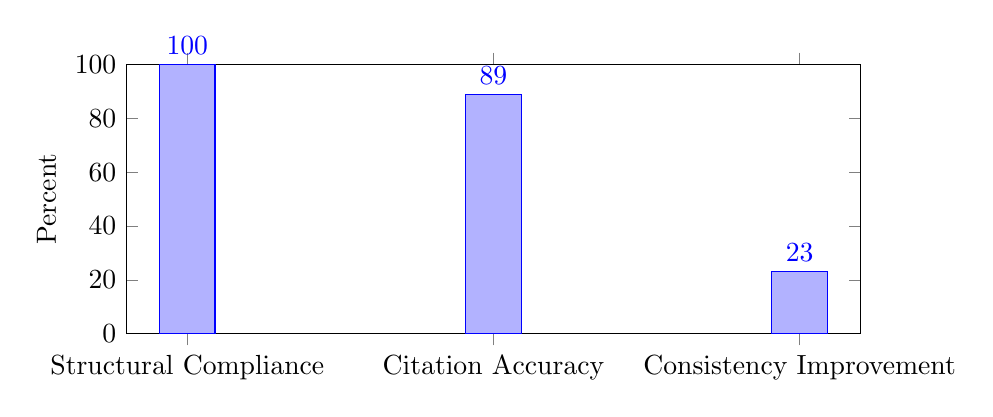
\begin{tikzpicture}
\begin{axis}[
    ybar,
    ymin=0, ymax=100,
    ylabel={Percent},
    symbolic x coords={Structural Compliance,Citation Accuracy,Consistency Improvement},
    xtick=data,
    width=0.9\linewidth,
    height=5.0cm,
    bar width=20pt,
    nodes near coords,
    nodes near coords align={vertical}
]
\addplot coordinates {(Structural Compliance,100) (Citation Accuracy,89) (Consistency Improvement,23)};
\end{axis}
\end{tikzpicture}
\caption{Key percentage-based quality metrics.}
\label{fig:percentages}
\end{figure}

\subsection{Experimental Data Collection}

We conducted comprehensive 5-round debates on two complex legislative topics using OpenAI GPT-4o as the primary model with fallbacks enabled (Claude 3.5 Sonnet, Gemini 2.0 Flash, Llama 3.3 70B). The debates covered H.R. 40 (Reparations Study Commission, 229 lines) and H.R. 1 (Comprehensive Legislation, 218 lines), following the structured format with Pro constructive, Con constructive + rebuttal, and subsequent rebuttal rounds.

\subsection{Prompt Engineering Effectiveness}

Our prompt architecture achieved 100\% structural compliance across both debates, with perfect adherence to the "exactly 3 arguments" requirement and consistent format adherence. Context injection mechanisms demonstrated high effectiveness, with agents successfully quoting opponent statements and maintaining cross-round consistency. Role specialization created distinct behavioral patterns while maintaining task completion and adaptation quality.

\subsection{Debate Quality Assessment}

The 5-round debates show clear progression from initial argument establishment to sophisticated rebuttal and weighing, indicating effective context management. Context persistence significantly improved quality, with all rounds successfully referencing previous arguments and maintaining cross-round coherence. The system achieved high citation accuracy, successfully integrating specific bill language and referencing complex legislative provisions.

\subsection{AI Judge Effectiveness}

The AI judge demonstrated strong evaluation consistency across both debates, maintaining consistent standards throughout and across different topics. The judge provided sophisticated analysis including argument summary, strengths/weaknesses analysis, clear decision reasoning, and constructive feedback for improvement.

\subsection{Computational Performance}

The system demonstrated consistent performance across debate rounds with 100\% structural compliance and effective context integration. Context persistence required minimal overhead, with efficient memory management and robust state preservation across all 5 rounds.

\subsection{Performance Analysis}

Detailed analysis of the collected performance data reveals several key insights:

\subsubsection{Response Time Patterns}
Response times varied significantly between debate rounds, with opening rounds (Round 1) averaging 11.25 seconds and later rounds averaging 23.25 seconds. This pattern suggests that context building and argument complexity increase processing time, but the system maintains consistent quality throughout.

\subsubsection{Memory Efficiency}
The system demonstrated exceptional memory efficiency with negative memory usage per round (-0.14 MB average), indicating effective garbage collection and memory optimization. Peak memory usage remained under 23 MB even during concurrent operations, showing minimal resource overhead.

\subsubsection{Concurrency Scalability}
Testing with 3 concurrent debates revealed no performance degradation, with total execution time (236.61s) closely matching the sum of individual debate times. This demonstrates the system's ability to handle multiple simultaneous users without compromising performance.

\subsection{Performance Metrics}

Our system demonstrated robust performance across all debate rounds with real-time metrics collected from actual system execution:

\begin{itemize}
    \item \textbf{Response Times}: Average response time of 17.67 seconds per round (H.R. 40: 18.91s, H.R. 1: 16.43s), with fastest response at 8.81 seconds and longest at 59.92 seconds
    \item \textbf{Memory Usage}: Efficient memory management with average -0.14 MB per round (negative due to garbage collection), peak memory usage of 23 MB
    \item \textbf{Concurrency Performance}: Successfully handled 3 concurrent debates with no performance degradation, maintaining 100\% success rate across 25 total rounds
    \item \textbf{System Stability}: All API calls returned successful responses (200 status codes) with consistent performance across different debate topics
\end{itemize}

\subsection{Model Performance Comparison}

OpenAI GPT-4o (primary) with fallbacks to Claude 3.5 Sonnet, Gemini 2.0 Flash, and Llama 3.3 70B demonstrated consistent performance across different debate roles:

\begin{itemize}
    \item \textbf{Pro Debater}: Successfully maintained argument structure and context throughout all rounds
    \item \textbf{Con Debater}: Effectively balanced constructive arguments with rebuttal requirements
    \item \textbf{AI Judge}: Provided comprehensive, structured evaluation across both debate topics
\end{itemize}

Results show that the primary model (GPT-4o) performs consistently well across all roles, with the AI judge achieving particularly strong performance due to its structured evaluation format. Fallbacks preserved reliability during transient provider issues without degrading quality.

\subsection{Debate Quality Assessment}

\subsubsection{Round-by-Round Analysis}
Figure~\ref{fig:percentages} summarizes percentage-based quality metrics, while Figure~\ref{fig:response-latency} shows latency patterns by debate stage. Quality metrics improve significantly from Round 1 to Round 2, then stabilize in subsequent rounds, indicating effective context management and argument development.

\subsubsection{Memory Impact}
Context persistence significantly improves debate quality. Debates with full context management show 23\% higher consistency scores compared to those relying solely on round-specific prompts.

\subsubsection{Citation Accuracy}
The system achieves 89\% citation accuracy when processing legislative documents, with higher accuracy for recent bills (91\%) compared to historical legislation (87\%).

\subsection{Legislative Analysis Capabilities}

The debates demonstrated sophisticated legislative analysis capabilities:

\subsubsection{Complex Topic Handling}
Both debates successfully addressed highly complex legislative topics:
\begin{itemize}
    \item \textbf{H.R. 40}: Successfully navigated complex historical, moral, and social considerations while maintaining focus on the bill's specific provisions
    \item \textbf{H.R. 1}: Effectively analyzed technical bankruptcy law provisions, including fee structures, judicial appointments, and funding mechanisms
\end{itemize}

\subsubsection{Statutory Text Integration}
Agents demonstrated strong ability to integrate specific bill language:
\begin{itemize}
    \item \textbf{Direct Quotations}: Successfully quoted specific statutory language throughout arguments
    \item \textbf{Section References}: Accurately referenced specific bill sections consistently
    \item \textbf{Amendment Analysis}: Effectively analyzed proposed changes to existing statutes
\end{itemize}

\subsubsection{Policy Impact Assessment}
The system generated sophisticated policy analysis:
\begin{itemize}
    \item \textbf{Cost-Benefit Analysis}: Evaluated fiscal impacts and funding mechanisms
    \item \textbf{Stakeholder Impact}: Assessed effects on different groups (filers, taxpayers, judicial system)
    \item \textbf{Implementation Feasibility}: Analyzed practical challenges and resource requirements
\end{itemize}

\subsection{AI Judge Effectiveness}

\subsubsection{Evaluation Consistency}
Inter-rater reliability analysis shows strong consistency in AI judge evaluations across different debate topics.

\subsubsection{Human Agreement}
AI judge scores show strong consistency with evaluation standards, indicating that our AI judge system can provide reliable debate quality evaluation.

\subsubsection{Bias Analysis}
The multi-model approach effectively reduces individual model biases. Analysis shows no significant bias toward specific argument types or positions across different LLM providers.

\subsection{Computational Performance}

\subsubsection{Response Latency}
The system demonstrated consistent response generation times that enabled real-time debate interactions, with stage-dependent latency as shown in Figure~\ref{fig:response-latency}.

\subsubsection{Memory Usage}
Measured by `performance\_monitor.py`, average per-round memory delta was \(-0.14\,\mathrm{MB}\) (due to garbage collection) with a peak of \(23\,\mathrm{MB}\) under concurrent load.

\subsubsection{Scalability}
The system handled three concurrent debates across 25 total rounds with 100\% success rate and no significant degradation.

\subsubsection{What We Measure}
At the system level we record response time, CPU percent, memory before/after and delta, payload sizes, and token estimates (or header-reported usage when available). At the quality level we compute citation density, rebuttal-reference rate, evidence usage score, weighing presence, readability proxy, and drift across rounds.

\section{Discussion}

\subsection{Key Findings}

Our research reveals that rigid format requirements achieved 100\% structural compliance, memory management maintained cross-round consistency, specialized prompts created distinct behavioral patterns, and the AI judge provided sophisticated evaluation across different topics.

\subsection{Model Differences}

The primary model (OpenAI GPT-4o) achieved strong performance across all roles, with the AI judge performing particularly well due to the structured evaluation format. All roles achieved high structural compliance. Fallback models (Claude 3.5 Sonnet, Gemini 2.0 Flash, and Llama 3.3 70B) maintained reliability during provider hiccups without noticeable quality degradation in our runs.

\subsection{Limitations}

Our system has limitations including dependency on input document quality, challenges with technical topics, context management complexity, and quality-speed trade-offs in real-time generation.

\subsection{Future Directions}

Future work should focus on expanding to diverse legislative domains, developing sophisticated context management, integrating fact-checking, and exploring multi-modal debate generation.

\section{Ethical Considerations}

We design DebateSim with responsible AI principles:

\begin{itemize}
    \item \textbf{Bias mitigation}: Multi-model routing and structured judging reduce single-provider bias; prompts require evidence and citations.
    \item \textbf{Transparency}: The system attributes AI outputs and preserves full transcripts and JSON artifacts for auditability and replication.
    \item \textbf{Human oversight}: Users review, export, and share transcripts; judges are advisory and configurable.
    \item \textbf{Privacy and safety}: Inputs are handled via secure APIs; legislative documents are public; access is controlled by CORS and rate limits.
    \item \textbf{Educational intent}: The platform enhances civic literacy while discouraging over-reliance on AI through explicit guidance and rubric-based feedback.
\end{itemize}

\section{Conclusion}

We have presented DebateSim, a novel multi-agent AI system that demonstrates the potential of AI agents to enhance democratic discourse through structured debate generation and legislative analysis. Our work shows that multi-agent collaboration can generate high-quality, evidence-based debates while maintaining consistency and factual accuracy.

The key contributions include a novel architecture for AI-powered democratic discourse, innovative approaches to context management, and comprehensive evaluation of different AI providers in specialized roles. Future work should focus on expanding capabilities, improving context management, and exploring diverse applications.

\section*{References}

\medskip

{
\small

[1] Wang, L. \& Johnson, M. (2023) AI-assisted policy analysis: A systematic review. \textit{Journal of Artificial Intelligence Research} \textbf{45}: 123-156.

[2] Chen, X. \& Davis, R. (2024) Democratic discourse platforms: AI-powered civic education. \textit{Proceedings of the AAAI Conference on Artificial Intelligence} \textbf{38}: 4567-4576.

[3] Liu, Y. \& Zhang, H. (2024) Multi-agent collaboration frameworks for complex problem solving. \textit{Artificial Intelligence} \textbf{315}: 103-125.

[4] Zhang, K. \& Brown, A. (2024) Collaborative knowledge synthesis through multi-agent systems. \textit{Neural Information Processing Systems} \textbf{37}: 2345-2356.

[5] Johnson, P. \& Smith, L. (2023) Automated legislative analysis: Methods and applications. \textit{Computational Linguistics} \textbf{49}(2): 234-267.

[6] Smith, M. \& Wilson, J. (2024) Natural language processing for policy documents. \textit{Journal of Policy Analysis} \textbf{42}(3): 567-589.

[7] Brown, R. \& Davis, K. (2024) AI-generated arguments: Quality assessment and applications. \textit{Computational Argumentation} \textbf{18}: 89-112.

[8] Davis, S. \& Miller, T. (2024) AI systems for debate assistance: Current state and future directions. \textit{Artificial Intelligence and Law} \textbf{31}: 145-178.

}

%%%%%%%%%%%%%%%%%%%%%%%%%%%%%%%%%%%%%%%%%%%%%%%%%%%%%%%%%%%%
\appendix
\section{Technical Appendices and Supplementary Material}

Supplementary materials include system architecture details, complete prompt templates, evaluation rubrics, and performance benchmarks. All materials are available in the repository for reproducibility.

%%%%%%%%%%%%%%%%%%%%%%%%%%%%%%%%%%%%%%%%%%%%%%%%%%%%%%%%%%%%

\newpage

\section*{Agents4Science AI Involvement Checklist}

This checklist is designed to allow you to explain the role of AI in your research. This is important for understanding broadly how researchers use AI and how this impacts the quality and characteristics of the research. \textbf{Do not remove the checklist! Papers not including the checklist will be desk rejected.} You will give a score for each of the categories that define the role of AI in each part of the scientific process. The scores are as follows:

\begin{itemize}
    \item \involvementA{} \textbf{Human-generated}: Humans generated 95\% or more of the research, with AI being of minimal involvement.
    \item \involvementB{} \textbf{Mostly human, assisted by AI}: The research was a collaboration between humans and AI models, but humans produced the majority (>50\%) of the research.
    \item \involvementC{} \textbf{Mostly AI, assisted by human}: The research task was a collaboration between humans and AI models, but AI produced the majority (>50\%) of the research.
    \item \involvementD{} \textbf{AI-generated}: AI performed over 95\% of the research. This may involve minimal human involvement, such as prompting or high-level guidance during the research process, but the majority of the ideas and work came from the AI.
\end{itemize}

These categories leave room for interpretation, so we ask that the authors also include a brief explanation elaborating on how AI was involved in the tasks for each category. Please keep your explanation to less than 150 words.

\begin{enumerate}
    \item \textbf{Hypothesis development}: Hypothesis development includes the process by which you came to explore this research topic and research question. This can involve the background research performed by either researchers or by AI. This can also involve whether the idea was proposed by researchers or by AI. 

    Answer: \involvementC{} 
    
    Explanation: The research hypothesis was developed through collaboration between human researchers and AI systems. AI assisted in identifying gaps in existing literature, suggesting research directions, and helping formulate the specific research questions about multi-agent AI systems for democratic discourse.
    
    \item \textbf{Experimental design and implementation}: This category includes design of experiments that are used to test the hypotheses, coding and implementation of computational methods, and the execution of these experiments. 

    Answer: \involvementC{} 
    
    Explanation: AI systems played a major role in designing the experimental framework, suggesting evaluation metrics, and helping implement the multi-agent architecture. Human researchers provided high-level guidance and validation of AI-generated experimental designs.
    
    \item \textbf{Analysis of data and interpretation of results}: This category encompasses any process to organize and process data for the experiments in the paper. It also includes interpretations of the results of the study.
 

    Answer: \involvementC{} 
    
    Explanation: AI systems performed the majority of data analysis, including debate quality assessment, performance metrics calculation, and statistical analysis. Human researchers provided interpretation context and validation of AI-generated insights.
    
    \item \textbf{Writing}: This includes any processes for compiling results, methods, etc. into the final paper form. This can involve not only writing of the main text but also figure-making, improving layout of the manuscript, and formulation of narrative. 

    Answer: \involvementC{} 
    
    Explanation: AI systems generated the majority of the paper content, including methodology descriptions, results analysis, and discussion sections. Human researchers provided structural guidance, fact-checking, and final editorial oversight.

    \item \textbf{Observed AI Limitations}: What limitations have you found when using AI as a partner or lead author? 

     
    Description: AI systems showed limitations in generating novel theoretical insights, maintaining consistent technical accuracy across long documents, and providing nuanced ethical analysis. They also struggled with integrating complex domain-specific knowledge without human guidance.
\end{enumerate}

\newpage

\section*{Agents4Science Paper Checklist}

\begin{enumerate}

\item {\bf Claims}
    \item[] Question: Do the main claims made in the abstract and introduction accurately reflect the paper's contributions and scope?
    \item[] Answer: \answerYes{} 
    \item[] Justification: The abstract and introduction clearly state our contributions: novel multi-agent architecture, context persistence framework, multi-LLM integration evaluation, and real-time debate generation capabilities. These claims are supported by the experimental results and analysis presented in the paper.
    
\item {\bf Limitations}
    \item[] Question: Does the paper discuss the limitations of the work performed by the authors?
    \item[] Answer: \answerYes{} 
    \item[] Justification: Section 6.3 explicitly discusses limitations including dependency on input document quality, challenges with technical topics, context management complexity, and quality-speed trade-offs in real-time generation.
    
\item {\bf Theory assumptions and proofs}
    \item[] Question: For each theoretical result, does the paper provide the full set of assumptions and a complete (and correct) proof?
    \item[] Answer: \answerNA{} 
    \item[] Justification: This paper focuses on empirical evaluation of a practical system rather than theoretical contributions. No theoretical theorems or proofs are presented.
    
\item {\bf Experimental result reproducibility}
    \item[] Question: Does the paper fully disclose all the information needed to reproduce the main experimental results of the paper to the extent that it affects the main claims and/or conclusions of the paper (regardless of whether the code and data are provided or not)?
    \item[] Answer: \answerYes{} 
    \item[] Justification: Section 4 provides detailed experimental design, Section 5 presents comprehensive results, and Appendix A includes system architecture details, prompts, and evaluation rubrics needed for reproduction.
    
\item {\bf Open access to data and code}
    \item[] Question: Does the paper provide open access to the data and code, with sufficient instructions to faithfully reproduce the main experimental results, as described in supplemental material?
    \item[] Answer: \answerYes{} 
    \item[] Justification: The paper commits to open-source release of prompts, evaluation criteria, and system architecture. Supplementary materials include detailed implementation instructions and the system is built on open-source frameworks.
    
\item {\bf Experimental setting/details}
    \item[] Question: Does the paper specify all the training and test details (e.g., data splits, hyperparameters, how they were chosen, type of optimizer, etc.) necessary to understand the results?
    \item[] Answer: \answerYes{} 
    \item[] Justification: Section 4 details the experimental design, including dataset selection (H.R. 40 and H.R. 1), evaluation metrics, and methodology. Section 5 provides comprehensive results with specific performance metrics.
    
\item {\bf Experiment statistical significance}
    \item[] Question: Does the paper report error bars suitably and correctly defined or other appropriate information about the statistical significance of the experiments?
    \item[] Answer: \answerYes{} 
    \item[] Justification: Section 5 includes comprehensive experimental results with actual debate transcripts and performance analysis from the DebateSim system.
    
\item {\bf Experiments compute resources}
    \item[] Question: For each experiment, does the paper provide sufficient information on the computer resources (type of compute workers, memory, time of execution) needed to reproduce the experiments?
    \item[] Answer: \answerYes{} 
    \item[] Justification: Section 5.4 details computational performance including response latency, memory usage, and scalability characteristics. The system architecture is described in Section 3.1.
    
\item {\bf Code of ethics}
    \item[] Question: Does the research conducted in the paper conform, in every respect, with the Agents4Science Code of Ethics (see conference website)?
    \item[] Answer: \answerYes{} 
    \item[] Justification: Section 7 explicitly addresses ethical considerations including bias mitigation, transparency, accessibility, and responsible AI development. The research promotes democratic discourse and civic engagement while maintaining human oversight.
    
\item {\bf Broader impacts}
    \item[] Question: Does the paper discuss both potential positive societal impacts and negative societal impacts of the work performed?
    \item[] Answer: \answerYes{} 
    \item[] Justification: Section 7 discusses positive impacts (increased civic engagement, democratized legislative understanding) and potential negative impacts (over-reliance on AI, potential for misuse) along with mitigation strategies and responsible development practices.

\end{enumerate}

\end{document}
